\section{Experiments}\label{sec:experiments}

We performed experiments on MNIST handwritten digits \citep{LeCun1998}, Fashion-MNIST images of clothing \citep{Xiao2017}, synthetic time series of linear interpolations of those images, time series from a chaotic dynamical system and real world medical data from the \emph{eICU Collaborative Research Database} \citep{Goldberger2000}.
If not otherwise noted, we use the same architecture for all experiments, sometimes including the latent probabilistic model (\emph{SOM-VAE\_prob}) and sometimes excluding it (\emph{SOM-VAE}).
For model implementation details, we refer to the appendix (Sec.~\ref{sec:implementation})\footnote{Our code is available at \url{https://github.com/ratschlab/SOM-VAE}.}.

We found that our method achieves a superior clustering performance compared to other methods.
We also show that we can learn a temporal probabilistic model concurrently with the clustering, which is on par with the maximum likelihood solution, while improving the clustering performance.
Moreover, we can learn interpretable state representations of a chaotic dynamical system and discover patterns in real medical data.


\subsection{Clustering on MNIST and Fashion-MNIST}\label{sec:clustering_benchmark}

In order to test the clustering component of the SOM-VAE, we performed experiments on MNIST and Fashion-MNIST.
We compare our model (including different adjustments to the loss function) against k-means \citep{Lloyd1982} (\texttt{sklearn}-package \citep{Pedregosa2011}), the VQ-VAE \citep{Oord2017}, a standard implementation of a SOM (\texttt{minisom}-package \citep{Vettigli2017}) and our version of a GB-SOM (gradient-based SOM), which is a SOM-VAE where the encoder and decoder are set to be identity functions.
The k-means algorithm was initialized using k-means++ \citep{Arthur2007-rk}.
To ensure comparability of the performance measures, we used the same number of clusters (i.e.\ the same $k$) for all the methods.

The results of the experiment in terms of purity and normalized mutual information (NMI) are shown in Table~\ref{tab:performance}.
The SOM-VAE outperforms the other methods w.r.t.\ the clustering performance measures.
It should be noted here that while k-means is a strong baseline, it is not density matching, i.e.\ the density of cluster centers is not proportional to the density of data points.
Hence, the representation of data in a space induced by the k-means clusters can be misleading.

As argued in the appendix (Sec.~\ref{sec:clustering_performance}), NMI is a more balanced measure for clustering performance than purity.
If one uses 512 embeddings in the SOM, one gets a lower NMI due to the penalty term for the number of clusters, but it yields an interpretable two-dimensional representation of the manifolds of MNIST (Fig.~\ref{fig:MNIST_SOM_selection}, Supp.~Fig.~\ref{fig:MNIST_SOM}) and Fashion-MNIST (Supp.\ Fig.~\ref{fig:FMNIST_SOM}).

\begin{figure}
    \centering
    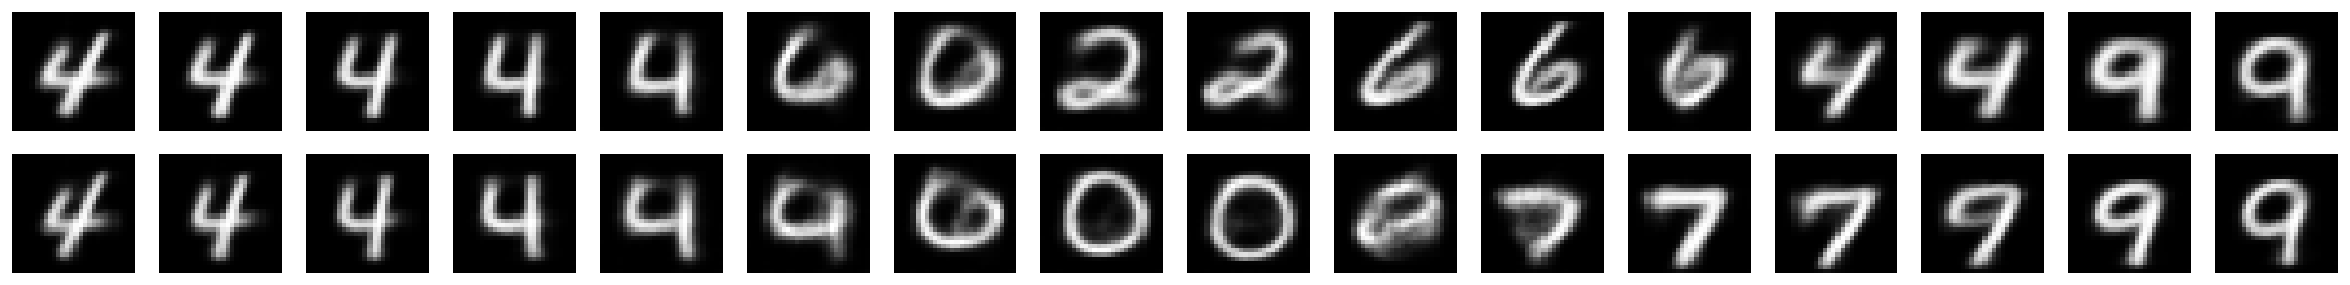
\includegraphics[width=0.9\textwidth]{MNIST_somvae_selection.pdf}
    \caption{Images generated from a section of the SOM-VAE's latent space with 512 embeddings trained on MNIST. It yields a discrete two-dimensional representation of the data manifold in the higher-dimensional latent space.}
    \label{fig:MNIST_SOM_selection}
\end{figure}

The experiment shows that the SOM in our architecture improves the clustering (SOM-VAE vs.\ VQ-VAE) and that the VAE does so as well (SOM-VAE vs.\ GB-SOM).
Both parts of the model therefore seem to be beneficial for our task.
It also becomes apparent that our reconstruction loss term on $z_e$ works better in practice than the gradient copying trick from the VQ-VAE (SOM-VAE vs.\ gradcopy), due to the reasons described in Section~\ref{sec:non-differentiability}.
If one removes the $z_e$ reconstruction loss and does not copy the gradients, the encoder network does not receive any gradient information any more and the learning fails completely (no\_grads).
Another interesting observation is that stochastically optimizing our SOM loss using Adam \citep{Kingma2015} seems to discover a more performant solution than the classical SOM algorithm (GB-SOM vs.\ minisom).
This could be due to the dependency of the step size on the distance between embeddings and encodings, as described in Section~\ref{sec:SOM-VAE}.
Since k-means seems to be the strongest competitor, we are including it as a reference baseline in the following experiments as well.


\begin{table}
    \centering
    \caption{Performance comparison of our method and some baselines in terms of purity and normalized mutual information on different benchmark data sets. The methods marked with an asterisk are variants of our proposed method. The values are the means of 10 runs and the respective standard errors. Each method was used to fit 16 embeddings/clusters.}
    \begin{tabular}{lrrrr}
        \toprule
         & \multicolumn{2}{c}{MNIST} & \multicolumn{2}{c}{Fashion-MNIST} \\
        \cmidrule(rl){2-3}
        \cmidrule(rl){4-5}
        Method & \multicolumn{1}{c}{Purity} & \multicolumn{1}{c}{NMI} & \multicolumn{1}{c}{Purity} & \multicolumn{1}{c}{NMI} \\
         \midrule
         k-means & 0.690 $\pm$ 0.000 & 0.541 $\pm$ 0.001 & 0.654 $\pm$ 0.001 & 0.545 $\pm$ 0.000 \\
         minisom & 0.406 $\pm$ 0.006 & 0.342 $\pm$ 0.012 & 0.413 $\pm$ 0.006 & 0.475 $\pm$ 0.002 \\
         GB-SOM & 0.653 $\pm$ 0.007 & 0.519 $\pm$ 0.005 & 0.606 $\pm$ 0.006 & 0.514 $\pm$ 0.004 \\
         VQ-VAE & 0.538 $\pm$ 0.067 & 0.409 $\pm$ 0.065 & 0.611 $\pm$ 0.006 & 0.517 $\pm$ 0.002 \\
         no\_grads* & 0.114 $\pm$ 0.000 & 0.001 $\pm$ 0.000 & 0.110 $\pm$ 0.009 & 0.018 $\pm$ 0.016 \\
         gradcopy* & 0.583 $\pm$ 0.004 & 0.436 $\pm$ 0.004 & 0.556 $\pm$ 0.008 & 0.444 $\pm$ 0.005 \\
         SOM-VAE* & \textbf{0.731 $\pm$ 0.004} & \textbf{0.594 $\pm$ 0.004} & \textbf{0.678 $\pm$ 0.005} & \textbf{0.590 $\pm$ 0.003} \\
         \bottomrule
    \end{tabular}
    \label{tab:performance}
\end{table}

\FloatBarrier

\subsection{Markov transition model on the discrete representations}

In order to test the probabilistic model in our architecture and its effect on the clustering, we generated synthetic time series data sets of (Fashion-)MNIST images being linearly interpolated into each other.
Each time series consists of 64 frames, starting with one image from \mbox{(Fashion-)MNIST} and smoothly changing sequentially into four other images over the length of the time course.

After training the model on these data, we constructed the maximum likelihood estimate (MLE) for the Markov model's transition matrix by fixing all the weights in the SOM-VAE and making another pass over the training set, counting all the observed transitions.
This MLE transition matrix reaches a negative log likelihood of $0.24$, while our transition matrix, which is learned concurrently with the architecture, yields $0.25$.
Our model is therefore on par with the MLE solution.

Comparing these results with the clustering performance on the standard MNIST and Fashion-MNIST test sets, we observe that the performance in terms of NMI is not impaired by the inclusion of the probabilistic model into the architecture (Tab.~\ref{tab:performance_prob}).
On the contrary, the probabilistic model even slightly increases the performance on Fashion-MNIST.
Note that we are using 64 embeddings in this experiment instead of 16, leading to a higher clustering performance in terms of purity, but a slightly lower performance in terms of NMI compared to Table~\ref{tab:performance}.
This shows again that the measure of purity has to be interpreted with care when comparing different experimental setups and that therefore the normalized mutual information should be preferred to make quantitative arguments.

This experiment shows that we can indeed fit a valid probabilistic transition model concurrently with the SOM-VAE training, while at the same time not hurting the clustering performance.
It also shows that for certain types of data the clustering performance can even be improved by the probabilistic model (see Sec.~\ref{sec:probabilistic_model}).

\begin{table}
    \centering
    \caption{Performance comparison of the SOM-VAE with and without latent Markov model (SOM-VAE-prob) against k-means in terms of purity and normalized mutual information on different benchmark data sets. The values are the means of 10 runs and the respective standard errors. Each method is used to fit 64 embeddings/clusters.}
    \begin{tabular}{lrrrr}
        \toprule
         & \multicolumn{2}{c}{MNIST} & \multicolumn{2}{c}{Fashion-MNIST} \\
        \cmidrule(rl){2-3}
        \cmidrule(rl){4-5}
        Method & \multicolumn{1}{c}{Purity} & \multicolumn{1}{c}{NMI} & \multicolumn{1}{c}{Purity} & \multicolumn{1}{c}{NMI} \\
         \midrule
         k-means & 0.791 $\pm$ 0.005 & 0.537 $\pm$ 0.001 & 0.703 $\pm$ 0.002 & 0.492 $\pm$ 0.001 \\
         SOM-VAE & \textbf{0.868 $\pm$ 0.003} & \textbf{0.595 $\pm$ 0.002} & \textbf{0.739 $\pm$ 0.002} & 0.520 $\pm$ 0.002 \\
         SOM-VAE-prob & 0.858 $\pm$ 0.004 & \textbf{0.596 $\pm$ 0.001} & 0.724 $\pm$ 0.003 & \textbf{0.525 $\pm$ 0.002} \\
         \bottomrule
    \end{tabular}
    \label{tab:performance_prob}
\end{table}


\subsection{Interpretable representations of chaotic time series} \label{sec:lorenz}

In order to assess whether our model can learn an interpretable representation of more realistic chaotic time series, we train it on synthetic trajectories simulated from the famous \emph{Lorenz system} \citep{Lorenz1963}.
The Lorenz system is a good example for this assessment, since it offers two well defined macro-states (given by the attractor basins) which are occluded by some chaotic noise in the form of periodic fluctuations around the attractors.
A good interpretable representation should therefore learn to largely ignore the noise and model the changes between attractor basins.
For a review of the Lorenz system and details about the simulations and the performance measure, we refer to the appendix (Sec.~\ref{sec:lorenz_appendix}).

In order to compare the interpretability of the learned representations, we computed entropy distributions over simulated subtrajectories in the real system space, the attractor assignment space and the representation spaces for k-means and our model.
The computed entropy distributions over all subtrajectories in the test set are depicted in Figure~\ref{fig:lorenz}. 

\begin{figure}[h!]
    \centering
    \begin{subfigure}[t]{0.15\textwidth}
\centering
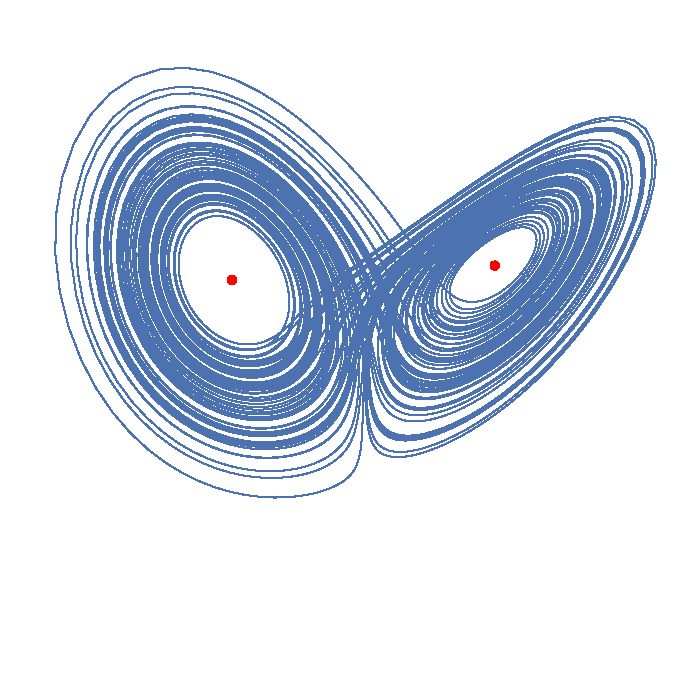
\includegraphics[scale=0.19]{lorenz/lorenz_attractor.pdf}
\subcaption{Lorenz attractor}
\end{subfigure}
    \begin{subfigure}[t]{0.15\textwidth}
\centering
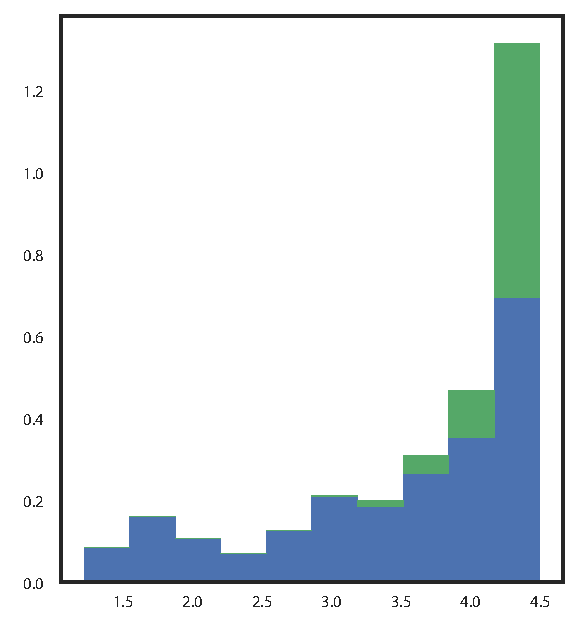
\includegraphics[scale=0.22]{lorenz/real_space.pdf}
\subcaption{Real space}
\label{fig:lorenz_real}
\end{subfigure}
    \begin{subfigure}[t]{0.15\textwidth}
\centering
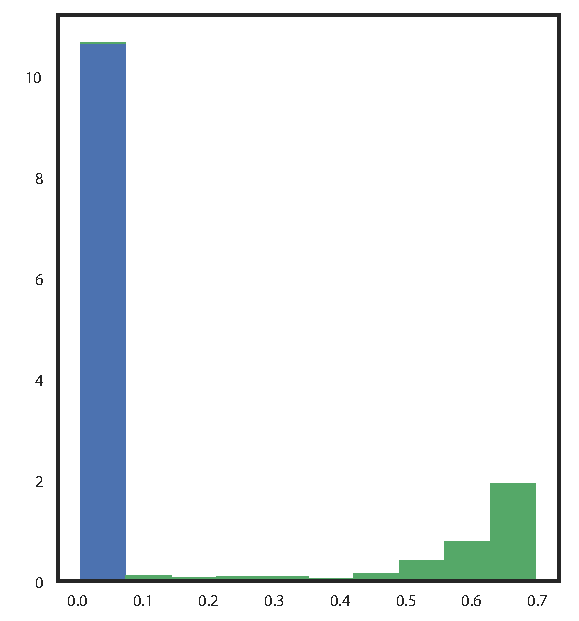
\includegraphics[scale=0.22]{lorenz/attractor_assignment.pdf}
\subcaption{Attractor assigment}
\label{fig:lorenz_assignment}
\end{subfigure}
    \begin{subfigure}[t]{0.15\textwidth}
\centering
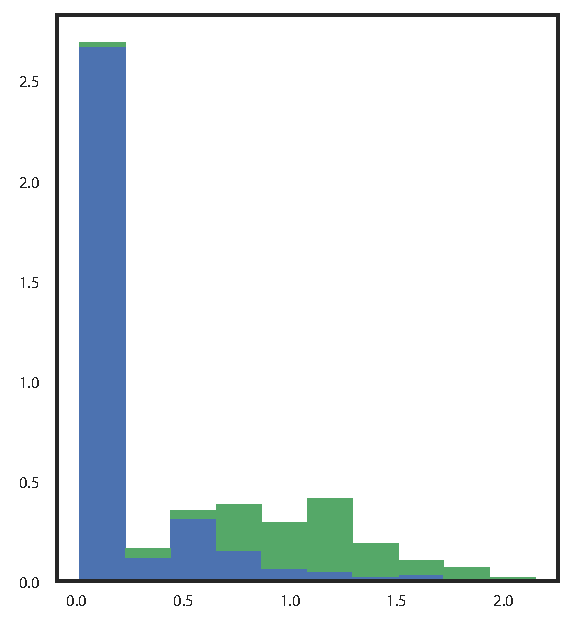
\includegraphics[scale=0.22]{lorenz/SOM_VAE.pdf}
\subcaption{SOM-VAE}
\label{fig:lorenz_somvae}
\end{subfigure}
    \begin{subfigure}[t]{0.15\textwidth}
\centering
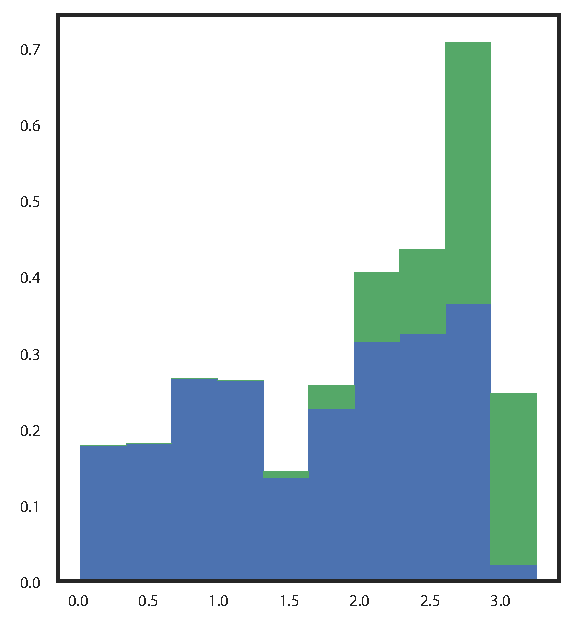
\includegraphics[scale=0.22]{lorenz/k_means.pdf}
\subcaption{k-means}
\label{fig:lorenz_kmeans}
\end{subfigure}
    \begin{subfigure}[t]{0.15\textwidth}
\centering
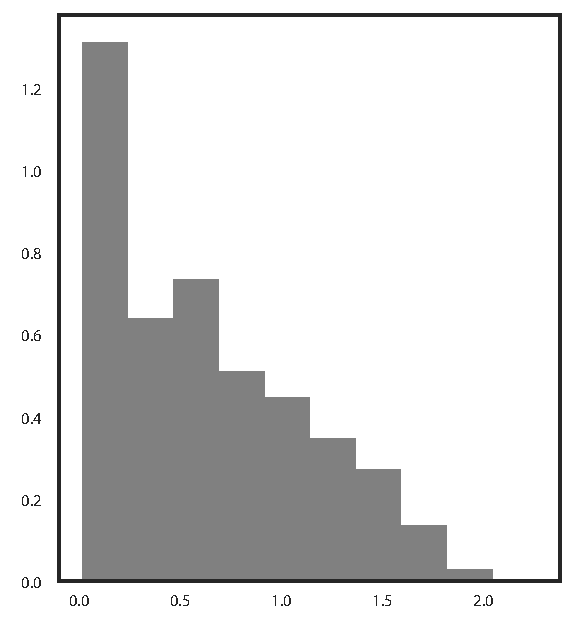
\includegraphics[scale=0.22]{lorenz/simulated.pdf}
\subcaption{Simulated trajectories}
\label{fig:lorenz_simulated}
\end{subfigure}

    \caption{Histograms of entropy distributions (entropy on the x-axes) over all Lorenz attractor subtrajectories [a] of 100 time steps length in our test set. Subtrajectories without a change in attractor basin are colored in blue, the ones where a change has taken place in green.}
    \label{fig:lorenz}
\end{figure}

The experiment shows that the SOM-VAE representations (Fig.~\ref{fig:lorenz_somvae}) are much closer in entropy to the ground-truth attractor basin assignments (Fig. \ref{fig:lorenz_assignment}) than the k-means representations (Fig. \ref{fig:lorenz_kmeans}).
For most of the subtrajectories without attractor basin change they assign a very low entropy, effectively ignoring the noise, while the k-means representations partially assign very high entropies to those trajectories.
In total, the k-means representations' entropy distribution is similar to the entropy distribution in the noisy system space (Fig.~\ref{fig:lorenz_real}).
The representations learned by the SOM-VAE are therefore more interpretable than the k-means representations with regard to this interpretability measure.
As could be expected from these figures, the SOM-VAE representation is also superior to the k-means one in terms of purity with respect to the attractor assignment ($0.979$ vs.\ $0.956$) as well as NMI ($0.577$ vs.\ $0.249$).

Finally, we use the learned probabilistic model on our SOM-VAE representations to sample new latent system trajectories and compute their entropies.
The distribution looks qualitatively similar to the one over real trajectories (Fig.\ \ref{fig:lorenz}), but our model slightly overestimates the attractor basin change probabilities, leading to a heavier tail of the distribution.

\FloatBarrier

\subsection{Learning representations of real medical time series}


In order to demonstrate interpretable representation learning on a complex real world task, we trained our model on vital sign time series measurements of intensive care unit (ICU) patients.
We analyze the performance of the resulting clustering w.r.t.\ the patients' future physiology states in Table \ref{tab:dynamic_performance_ICU}.
This can be seen as a way to assess the representations' informativeness for a downstream prediction task.
For details regarding the data selection and processing, we refer to the appendix (Sec.\ \ref{sec:ICU_appendix}).

\begin{table}
    \centering
    \caption{Performance comparison of our method with and without probabilistic model (SOM-VAE-prob and SOM-VAE) against k-means in terms of normalized mutual information on a challenging unsupervised prediction task on real eICU data. The dynamic endpoints are the maximum of the physiology score within the next 6, 12 or 24 hours (\emph{physiology\_6\_hours}, \emph{physiology\_12\_hours}, \emph{physiology\_24\_hours}). The values are the means of 10 runs and the respective standard errors. Each method is used to fit 64 embeddings/clusters.}
    \begin{tabular}{lrrr}
        \toprule
        Method & \multicolumn{1}{c}{physiology\_6\_hours} & \multicolumn{1}{c}{physiology\_12\_hours} & \multicolumn{1}{c}{physiology\_24\_hours} \\
         \midrule
         k-means & 0.0411 $\pm$ 0.0007 & 0.0384 $\pm$ 0.0006 & 0.0366 $\pm$ 0.0005 \\
         SOM-VAE & 0.0407 $\pm$ 0.0005 & 0.0376 $\pm$ 0.0004 & 0.0354 $\pm$ 0.0004 \\
         SOM-VAE-prob & \textbf{0.0474 $\pm$ 0.0006} & \textbf{0.0444 $\pm$ 0.0006} & \textbf{0.0421 $\pm$ 0.0005} \\
         \bottomrule
    \end{tabular}
    \label{tab:dynamic_performance_ICU}
\end{table}

Our full model (including the latent Markov model) performs best on the given tasks, i.e.\ better than k-means and also better than the SOM-VAE without probabilistic model.
This could be due to the noisiness of the medical data and the probabilistic model's smoothing tendency (see Sec.~\ref{sec:probabilistic_model}).

In order to qualitatively assess the interpretability of the probabilistic SOM-VAE, we analyzed the average future physiology score per cluster (Fig.~\ref{fig:heatmaps}).
Our model exhibits clusters where higher scores are enriched compared to the background level.
Moreover, these clusters form compact structures, facilitating interpretability.
We do not observe such interpretable structures in the other methods. For full results on acute physiology scores, an analogue experiment showing the 
future mortality risk associated with different regions of the map, and an analysis of enrichment for
particular physiological abnormalities, we refer to the appendix (Sec.\ \ref{subsec:detailed_icu}). 

As an illustrative example for data visualization using our method, we show the trajectories of two patients that start in the same state (Fig.~\ref{fig:patient_trajectories}).
The trajectories are plotted in the representation space of the probabilistic SOM-VAE and should thus be compared to the visualization in Figure~\ref{fig:ICU_representations}.
One patient (\emph{green}) stays in the regions of the map with low average physiology score and eventually gets discharged from the hospital healthily.
The other one (\emph{red}) moves into map regions with high average physiology score and ultimately dies.
Such knowledge could be helpful for doctors, who could determine the risk of a patient for certain deterioration scenarios from a glance at their trajectory in the SOM-VAE representation.

\begin{figure}
\centering
\begin{subfigure}[t]{0.22\textwidth}
\centering
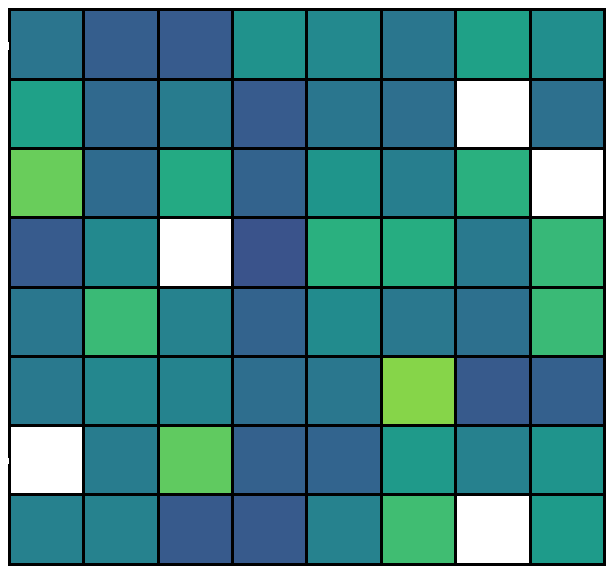
\includegraphics[scale=0.25]{k_means_full_score_24_enrichment_heatmap.pdf}
\subcaption{k-means}
\end{subfigure}
\begin{subfigure}[t]{0.22\textwidth}
\centering
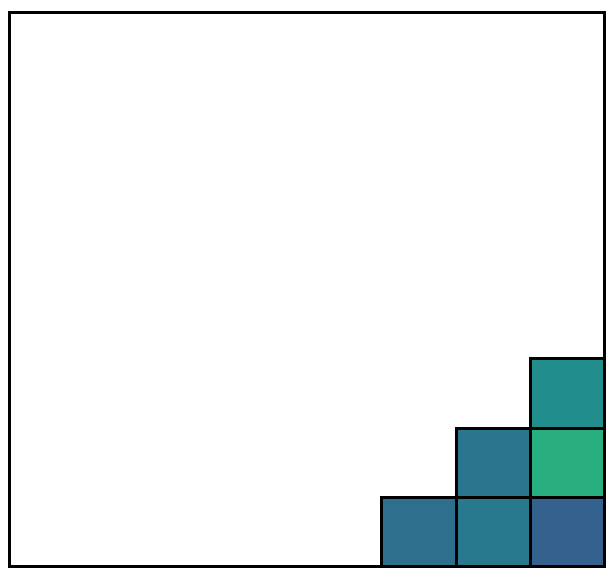
\includegraphics[scale=0.25]{vqvae_full_score_24_enrichment_heatmap.pdf}
\subcaption{VQ-VAE}
\end{subfigure}
\begin{subfigure}[t]{0.22\textwidth}
\centering
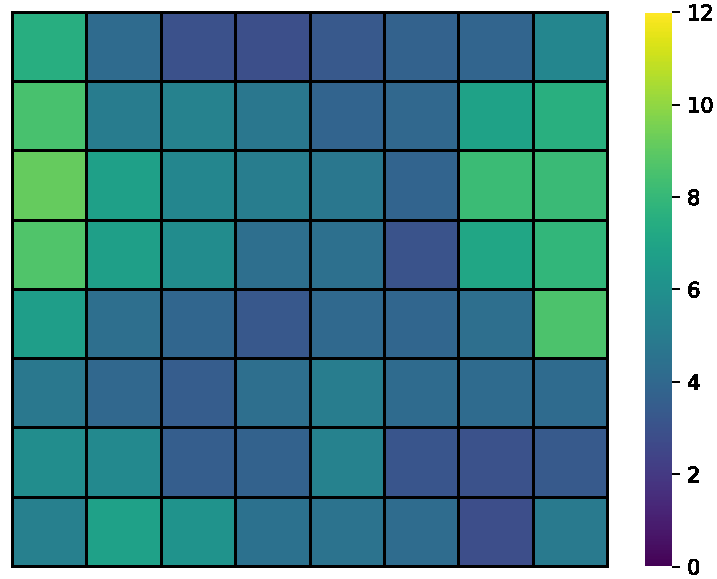
\includegraphics[scale=0.25]{somvae_prob_full_score_24_enrichment_heatmap.pdf}
\subcaption{SOM-VAE-prob}
\label{fig:ICU_representations}
\end{subfigure}
\begin{subfigure}[t]{0.22\textwidth}
\centering
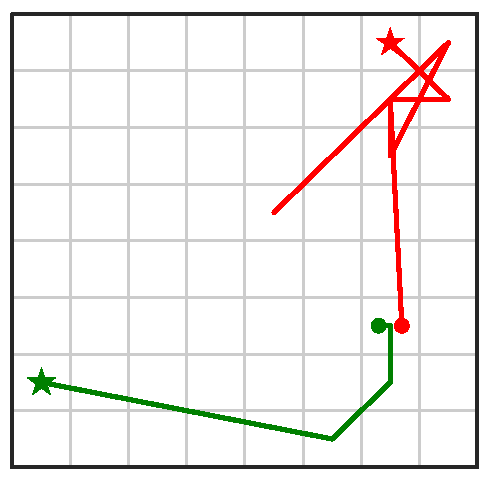
\includegraphics[scale=0.31]{patient_trajectory_example.pdf}
\subcaption{Patient trajectories}
\label{fig:patient_trajectories}
\end{subfigure}
\caption{Comparison of the patient state representations learned by different models. The clusters are colored by degree of patient abnormality as measured by a variant of the APACHE physiology score (more yellow means ``less healthy'').
White squares correspond to unused clusters, i.e.\ clusters that contain less than 0.1 percent of the data points.
Subfigure (d) shows two patient trajectories in the SOM-VAE-prob representation over their respective whole stays in the ICU.
The dots mark the ICU admission, the stars the discharge from the ICU (cured [green] or dead [red]).
It can be seen that our model is the only one that learns a topologically interpretable structure.
}
\label{fig:heatmaps}
\end{figure}


